% !TEX encoding = UTF-8 Unicode
\documentclass{beamer}

\usepackage{color}
\usepackage{url}
\usepackage[T2A]{fontenc}
\usepackage[utf8]{inputenc}
\usepackage{graphicx}
\usepackage[english,serbian]{babel}
\usepackage{chemfig}
\usepackage[version=3]{mhchem}
\usepackage{multicol}


\mode<presentation>
{
  \usetheme{Warsaw}       
  \usecolortheme{default} 
  \usefonttheme{serif}    
  \setbeamertemplate{navigation symbols}{}
  \setbeamertemplate{caption}[numbered]
} 


\definecolor{mygreen}{rgb}{0,0.6,0}
\definecolor{mygray}{rgb}{0.5,0.5,0.5}
\definecolor{mymauve}{rgb}{0.58,0,0.82}

\usepackage{listings}
\lstset{ 
  backgroundcolor=\color{white},
  basicstyle=\scriptsize\ttfamily,
  breakatwhitespace=false,
  breaklines=true,
  captionpos=b,
  commentstyle=\color{mygreen},
  deletekeywords={...},            
  escapeinside={\%*}{*)},          
  extendedchars=true,
  firstnumber=1,              
  frame=single,	                
  keepspaces=true,
  keywordstyle=\color{blue},     
  language=Python,                
  morekeywords={*,...},
  numbers=left, 
  numbersep=4pt,                  
  numberstyle=\tiny\color{mygray}, 
  rulecolor=\color{black},
  showspaces=false,
  showstringspaces=false,
  showtabs=false,
  stepnumber=1, 
  stringstyle=\color{mymauve},
  tabsize=1,
  title=\lstname
}
\usepackage{pgfpages}
\pgfpagesuselayout{resize to}[%
  physical paper width=8in, physical paper height=6in]

\title{F\# na .NET platformi}
\author{T.Todorov T.Garibović D.Nedeljković M.Vićentijević}
\date{\today}

\begin{document}
\begin{frame}
  \titlepage
\end{frame}

\begin{frame}{Pregled}
  \tableofcontents
\end{frame}

\section{Uvod}

\begin{frame}{Uvod}
\begin{itemize}
\item F\# je jezik koji danas ima veoma široku upotrebu
\item Nastao je iz ideje da se strogo tipizirani funkcionalni jezik preusmeri na .NET platformu
\item Autor jezika je Don Sajm (eng.~{\em Don Syme})
\item Pretežno je funkcionalan jezik, ali podržava još dosta programskih paradigmi
\item F\# ima jednostavnu sintaksu, a dovoljno moćnu i za složene matematičke probleme
\item Cilj rada je izdvajanje nekih specifičnih karakteristika
\end{itemize}
\end{frame}

\section{Nastanak i primena jezika F\#}
\subsection*{Poreklo i uticaj drugih jezika}
\begin{frame}{Poreklo i uticaj drugih jezika}

\begin{figure}
\begin{center}
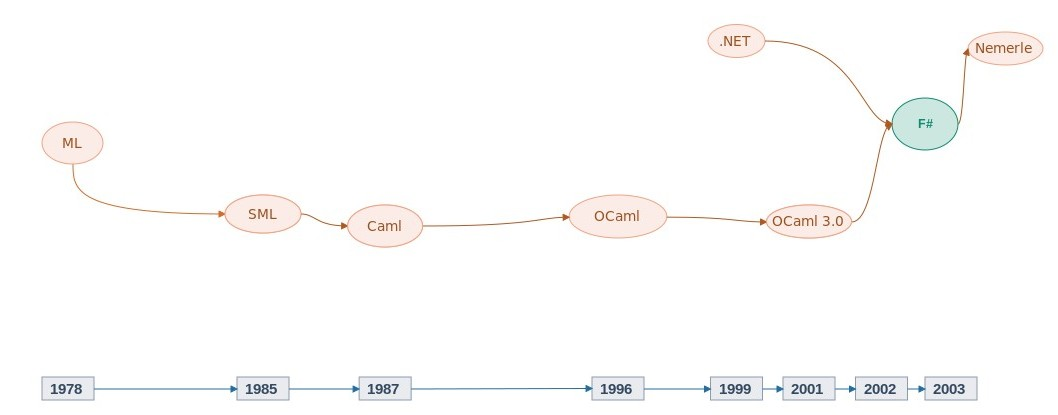
\includegraphics[scale=0.3]{stablo.jpg}
\end{center}
\caption{Razvojno stablo}
\end{figure}

\end{frame}

\subsection*{Primena i mogućnosti}
\begin{frame}{Primena i mogućnosti}

\begin{itemize}
\item Jednostavna sintaksa omogućava laku čitljivost koda
\item Jezik omogućava brzo generisanje prototipova
\item Kôd napisan u F\#-u lako može da se paralelizuje
\item Jezik ima primenu u oblastima: bioinformatika, baze podataka, statistika, finansijsko modelovanje, ...
\item Osim funkcionalnog, jezik F\#, podržava još neke tipove programiranja: imperativno, objektno-orjentisano, paralelno, distribuirano, asinhrono, veb programiranje, skript programiranje, ...
\item Koristi se na dosta operativnih sistema: Linux, MAC, Windows, Android, iOS, ...
\end{itemize}

\end{frame}

\section{Osobine i neke paradigme}
\subsection*{Osobine i specifičnosti jezika}
\begin{frame}{Osobine i specifičnosti}
\begin{center}

\textbf{Osobine:} ~~~~~~~~~~~~~~~~~~~~~~~~~~~~ \textbf{Specifičnosti:}
\end{center}
\begin{multicols}{2}
\begin{itemize}
  \item Bezbedan
  \item Funkcionalan
  \item Strogo tipiziran
  \item Automatski zaključuje tipove
  \item Kompatibilan
  \item Povratna vrednost if/else
  \item Opciono - return
  \item Ključne reči let i mutable
  \item Pattern matching
  \item Novi tip option type
\end{itemize}
\end{multicols}

\end{frame}

\subsection*{Funcionalna paradigma - Pattern matching}  
\begin{frame}[fragile]
\frametitle{Funcionalna paradigma - Pattern matching}


\begin{block}{Pattern matching}
Pattern matching je mehanizam koji koristi dekompoziciju i kontrolu toka podataka za poklapanje obrazaca koriščenjem navedene konstrukcije:
\textbf{ match ... with ...}
\end{block}
\begin{lstlisting}
let urlFilter url port =
 match (url,port) with
 | "http://www.control.org", 99 -> true
 | "http://www.kaos.org" , _ -> false
 | _, 86 -> true
 | _ -> false
\end{lstlisting} 

\end{frame}

\subsection*{Asinhrono i paralelno programiranje}
\begin{frame}[fragile]
\frametitle{Asinhrono i paralelno programiranje}

\begin{itemize}
\item \textbf{Asinhrono programiranje}
\begin{itemize}
	\item Opisuje programe i operacije koje se izvršavaju u pozadini i završavaju nakon nekog vremena
	\item Programe možemo pisati korišćenjem \textbf{APM} biblioteke
	\item APM deli asinhrone operacije na dve metode: BeginOperation i EndOperation
\end{itemize}

\item \textbf{Paralelno programiranje}
\begin{itemize}
	\item Na .NET 4.0 platformi se koristi \textbf{PFX} biblioteka čija je osnovna struktura \textbf{Task objekat}
	\item Zbog problema Task objekta sa deljenim podacima uvodi se zaključavanje podataka
	\item PFX biblioteka uvodi nove kolekcije System.Collections.Concurrent	
\end{itemize}
\end{itemize}



\end{frame}

\section{Radni okviri i instalacija}
\subsection*{Radni okvir - .NET framework}
\begin{frame}[fragile]
\frametitle{Radni okvir - .NET framework}

\begin{itemize}
\item \textbf{.NET platforma} je platforma koja podržava veliki broj različitih kompatabilnih jezika, programskih paradigmi ali i .NET radni okvir (eng.~{\em framework}).
\item .NET radni okvir je pojednostavio razvoj RP({\em Reactive Programming}) aplikacija ali i podržava veliki broj biblioteka i editora.
\item Temelj .NET platforme je zajednička jezička infrastruktura \textbf{CLI} ({\em Common Language Infrastructure)}.
\item Kodovi se prevode na \textbf{MSIL} ({\em Microsoft Intermediate Language}) asemblerski jezik.\\
\end{itemize}

\end{frame}

\subsection*{Radni okvir - .NET framework}
\begin{frame}[fragile]
\frametitle{Radni okvir - .NET framework}

\begin{itemize}
\item Implementacija MSIL-a na CLI kompajleru je brža i ima sledeće prednosti u odnosu na mašinski:
\begin{itemize}

	\item kompatibilnost među jezicima
	\item mogućnost rada na više platformi
	\item mašinska nezavisnost
\end{itemize}
\item Mogućnost automatskog prikupljanja smeća je još jedna prednost.
\end{itemize}

Još neki radni okviri: \textbf{veb} radni okviri({\em Suave, Fable, ASP.NET Core}...) i radni okviri za \textbf{testiranje veba} ({\em Web Testing, Frameworks, Unit Testing Libraries}...)
\end{frame}

\subsection*{Instalacija i pokretanje}
\begin{frame}[fragile]
\frametitle{Instalacija i pokretanje}

\begin{itemize}
\item Alati koji na \textbf{Windows-u} podržavaju F\# instaliraju se u nekoliko koraka:
	\begin{itemize}
	\item Visual Studio Code
	\item Visual studio
	\item JetBrains Rider
	\end{itemize}
\item Na \textbf{Linux-u} se instalacija vrši na isti način za sledece verzije:
	\begin{itemize}
	\item Ubuntu
	\item Mint
	\item Debian
	\end{itemize}
\item \begin{lstlisting}
sudo apt-get update
sudo apt-get install fsharp
\end{lstlisting}
\end{itemize}
\end{frame}


\section{F\# kroz primere}
\subsection*{Fizz Buzz}
\begin{frame}[fragile]
\frametitle{Fizz Buzz}
\begin{lstlisting}
let (|Fizz|Buzz|FizzBuzz|Other|) n =
    match (n % 3, n % 5) with
    | 0, 0 -> FizzBuzz
    | 0, _ -> Fizz
    | _, 0 -> Buzz
    | _ -> Other n

let fizzBuzz =
    function
    | Fizz -> "Fizz"
    | Buzz -> "Buzz"
    | FizzBuzz -> "FizzBuzz"
    | Other n -> n.ToString()

seq { 1..100 } |> Seq.map fizzBuzz|> Seq.iter (printfn "%s")
\end{lstlisting}

\end{frame}

\subsection*{Jedinica mere}
\begin{frame}[fragile]
\frametitle{Jedinica mere}

\begin{itemize}
  \item Pad orbitera poslatog na Mars 1999.
  \begin{itemize}
  	\item Uzrokovan činjenicom da je deo softvera koristio numeričke, a deo softvera engleske jedinice
  \end{itemize}
  \item Prevencija grešaka na osnovu konteksta primene
  \begin{itemize}
  	\item Numeričkim tipovima se pridružuju metapodaci
  	\item Kompajler na osnovu metapodataka proverava ispravnost
  \end{itemize}
  \item Jedinstveno svojstvo jezika F\#
  \item Primer definisanja jedinice mere  
\begin{lstlisting}
  [<Measure>] type cm
  [<Measure>] type inch  
\end{lstlisting}
\end{itemize}
\end{frame}

\subsection*{Jedinica mere}
\begin{frame}[fragile]
\frametitle{Jedinica mere}

\begin{lstlisting}
[<Measure>] type rsd
[<Measure>] type eur
[<Measure>] type hour
[<Measure>] type week
[<Measure>] type year

let hoursBilledPerWeek = 40.0<hour/week>
let weeksWorkedPerYear = 35.0<week/year>
let rsdPerHour = 1000.0<rsd/hour>
let exchangeRate = 0.008547<eur/rsd>

let eurPerYear = rsdPerHour * hoursBilledPerWeek * weeksWorkedPerYear * exchangeRate
let bonus = 500.0<eur/year>

printfn "%f" (eurPerYear + bonus)
\end{lstlisting}
\end{frame}

\section{Literatura}

\begin{frame}{Literatura}
 \begin{itemize}
	\item Don Syme, The Early History of F\# 	
  	\item Smith Chris, Programing F\# O’Reilly (2009)
  	\item Antonio Cisternino, Don Syme, Adam Granicz, Expert F\# (2007)
  	\item Jon Harrop, F\# for Scientists (2008)
  	\item \href{https://fsharp.org}{https://fsharp.org}
  \end{itemize}
 
\end{frame}

\section{}
\begin{frame}{}
 \begin{center}
 	\textbf {Hvala na pažnji!}
 \end{center}
\end{frame}

\end{document}